\chapter{Compact Graph for Query Transformation}
\label{sec:compact-graph-section}
Let $S\subseteq V$ be the Steiner set of vertices. Suppose $S'\subset S$ be any maximal subset of vertices with connectivity greater than that of $S$.  Observe that the entire set $S'$ will be mapped to a single node, say $\nu$, in the skeleton ${\cal H}_S$. In this section, we present the construction of a compact graph $G_{S'}$ such that any query \textsc{edge-contained}$(s,r,E_y)$ in graph $G$ can be efficiently transformed to a query \textsc{edge-contained}$(s,r,E_{y'})$ in graph $G_{S'}$ for any $s,r\in S'$.
% on which can answer \textsc{edge-contained}$(s,r,E_y)$ efficiently for any $s,r\in S'$ and any subset $E_y$ of edges emanating from $y\in V$.
\vspace{-2mm}
\section{Construction of Compact Graph \texorpdfstring{$G_{S'}$}{}}\label{sec:compact-graph}


The construction of $G_{S'}$ from the graph $G$, flesh ${\cal F}_S$ and skeleton ${\cal H}_S$ is a $2-$step process. In the 1st step, we contract the subcactuses neighbouring to node $\nu$ using the following procedure.
%We start with the original graph and then contract the subcactuses using the following procedure,

{\textsc{Contract-Subcactuses}}: For each tree-edge incident on $\nu$ (or cycle $c$ passing through $\nu$) in skeleton ${\cal H}_S$, remove the tree-edge (or the pair of edges from $c$ incident on $\nu$) to get 2 subcactuses. Compress all the terminal units of ${\cal F}_S$ that belong to the subcactus not containing $\nu$ into a single vertex. Moreover, compress all the stretched units with both endpoints within this subcactus into the same vertex.

In the quotient graph obtained after 1st step, each contracted subcactus defines a Steiner mincut. 
However, this graph may not necessarily be compact since there may be many stretched units that are not yet compressed. 
%Consider one such stretched unit $u$ and suppose
Let $u$ be any such unit and suppose
the path to which it is mapped in the skeleton is $P(\nu_1,\nu_2)$. If one of $\nu_1$ or $\nu_2$ is $\nu$, we can compress the stretched unit to the contracted vertex corresponding to the other endpoint. To handle the case when the subcactuses containing $\nu_1$ and $\nu_2$ are compressed to different vertices,
%The challenge is to tackle the case when subcactuses containing $\nu_1$ and $\nu_2$ are compressed to different vertices. 
% At first sight, it may seem appropriate to arbitrarily compress such stretched unit to one of these vertices. However, this approach won't guarantee that the contracted subcactus corresponds to a Steiner mincut. It can be explained as follows. Suppose $u_1,u_2$ and $u_3$ are three stretched units and there is a coherent path in ${\cal F}_S$ that passes through them in the order $\langle u_1,u_2,u_3 \rangle$. If we compress $u_2$ to one vertex and $u_1,u_3$ to another, the cut defined by either of these vertices will intersect the coherent path twice, and hence it will not be a Steiner mincut.
%To tackle this problem,
we define a total ordering on the set containing all tree-edges and cycles in the skeleton. The 2nd step uses this ordering to compress the stretched units as follows.
%Thenceforth, we contract each of the remaining stretched units to one of the contracted subcactus using the following procedure to get $G_{S'}$,


{\textsc{Contract-Stretched-Units}}: A stretched unit mapped to path $P(\nu_1,\nu_2)$, where $\nu_1\neq \nu \neq \nu_2$, is compressed to the contracted subcactus corresponding to lesser ordered cycle/tree-edge in which endpoints lie. If one of $\nu_1$ or $\nu_2$ is $\nu$, we compress it to the contracted subcactus corresponding to the cycle/tree-edge where other endpoint lies.

Figure \ref{fig:image-contraction} gives a nice illustration of the contraction procedure.

\begin{figure}
    \centering
    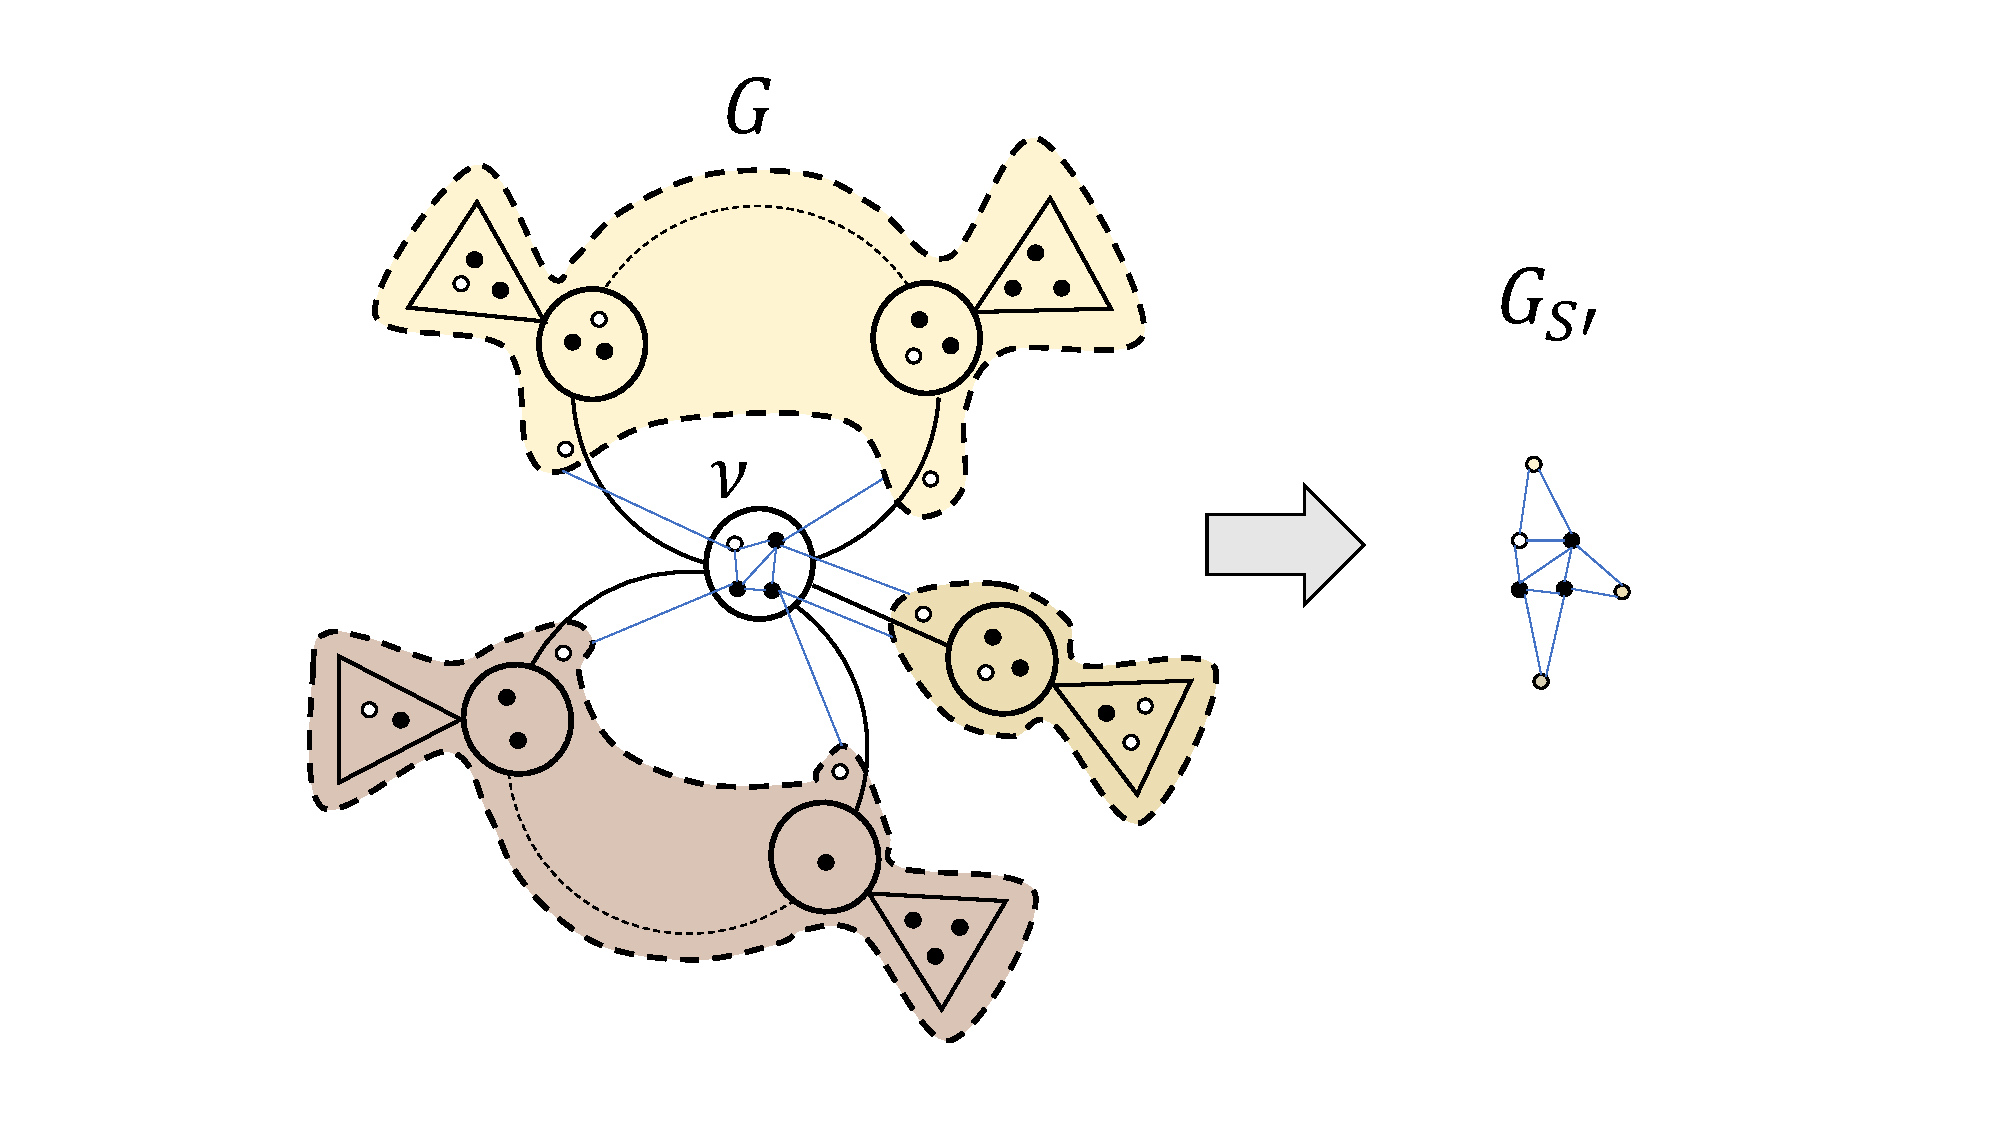
\includegraphics[width=\textwidth]{src/images/image_contraction.pdf}{}
    \caption{$2$-step contraction procedure to construct $G_{S'}$. We only show the vertices and relevant edges of graph along with the skeleton ${\cal H}_S$. Solid vertices belong to Steiner set $S$ and hollow vertices are non-Steiner vertices. All Steiner vertices inside node $\nu$ form the set $S'$.}
    \label{fig:image-contraction}
\end{figure}


Let $c$ be any cycle (or tree edge) passing through (incident on) $\nu$ in the skeleton
${\cal H}_S$. Let ${\cal D}_{s,t}$ be the strip corresponding to the sub-bunch defined by the structural edge(s) incident on $\nu$ by $c$.
Let $\nu$ be on the side of the source $\mathbf{s}$ in this strip.
Let ${\cal H}_S(c)$ be the subcactus formed by removing the structural edge(s) from $c$ incident on $\nu$ and not containing $\nu$. 
Recall that the subcactus ${\cal H}_S(c)$ was contracted into a vertex, say $v_c$, in the graph 
$G_{S'}$.
%Moreover, suppose $v_c$ is the contracted vertex corresponding to contracted subcactus ${\cal H}_S(c)$.
%Also, assume that $\nu$ is on the side of the source $\mathbf{s}$ in this sub-bunch.

\begin{lemma}
Let $u$ and $u'$ be any two non-terminal units in ${\cal D}_{s,t}$ such that none of them is compressed to $v_c$ in $G_{S'}$. If one of them is reachable from the other in the direction of ${\mathbf{s}}$, then both of them will be compressed to the same contracted vertex in $G_{S'}$.
%
%Let $u$ and $u'$ be any two non-terminal units in ${\cal D}_{s,t}$ such that $u'$ is reachable from $u$ in the direction of ${\mathbf{s}}$ and $u$ is not contracted to vertex $v_c$. $u'$ and $u$ will be compressed to the same contracted node in $G_{S'}$.
\label{lem:u-u'-in-G-nu}
\end{lemma}
\begin{proof}
Assume without loss of generality that $u'$ is reachable from $u$ in the direction of ${\mathbf{s}}$.
Let the proper paths associated with each of $u$ and $u'$ in ${\cal H}_S$ be $P(\nu_1,\nu_2)$ and $P(\nu_1',\nu_2')$ respectively. 
It follows from the construction of ${\cal D}_{s,t}$ that
$P(\nu_1,\nu_2)$ as well as $P(\nu_1',\nu_2')$ will pass through one of the structural edge(s) from $c$ on $\nu$. Without loss of generality,  assume that $P(\nu_1,\nu_2)$ passes through $e$. Since $P(\nu_1,\nu_2)$ is a proper path, this implies that this is the only structural edge in this cut (of skeleton) through which this path passes.
Since $u'$ is reachable from $u$ in flesh ${\cal F}_S$, so $P(\nu_1',\nu_2')$ will also have to pass through $e$ (from Lemma \ref{lem:path-extendable}).
It again follows from Lemma \ref{lem:path-extendable}, that $P(\nu_1,\nu_2)$ as well as $P(\nu_1',\nu_2')$ are subpaths of a path, say $P(\nu',\nu'')$, in skeleton
${\cal H}_S$. This combined with the above discussion establishes that $P(\nu',\nu'')$ has the structure shown in Figure \ref{fig:structure-of-p(nu',nu'')}.

Observe that any path in skeleton that passes through a node $\nu$ can intersect at most 2 cycles or tree-edges that are passing though $\nu$. We know that suffix of $P(\nu',\nu'')$ after $e$ lies in ${\cal H}_S(c)$, so the prefix upto $e$ must have endpoint in subcactus ${\cal H}_S(c')$ where $c'\neq c$. This implies that $u$ must be compressed to $v_{c'}$ because it is not compressed to $v_c$. Thus, $c'$ precedes $c$ in total order. It follows from the structure of path $P(\nu_1',\nu_2')$ that it will have an endpoint in ${\cal H}_S(c')$. Thus, $u'$ will be compressed to the same compressed vertex $v_{c'}$ in $G_{S'}$. This completes the proof.

\begin{figure}%[H]
\centering
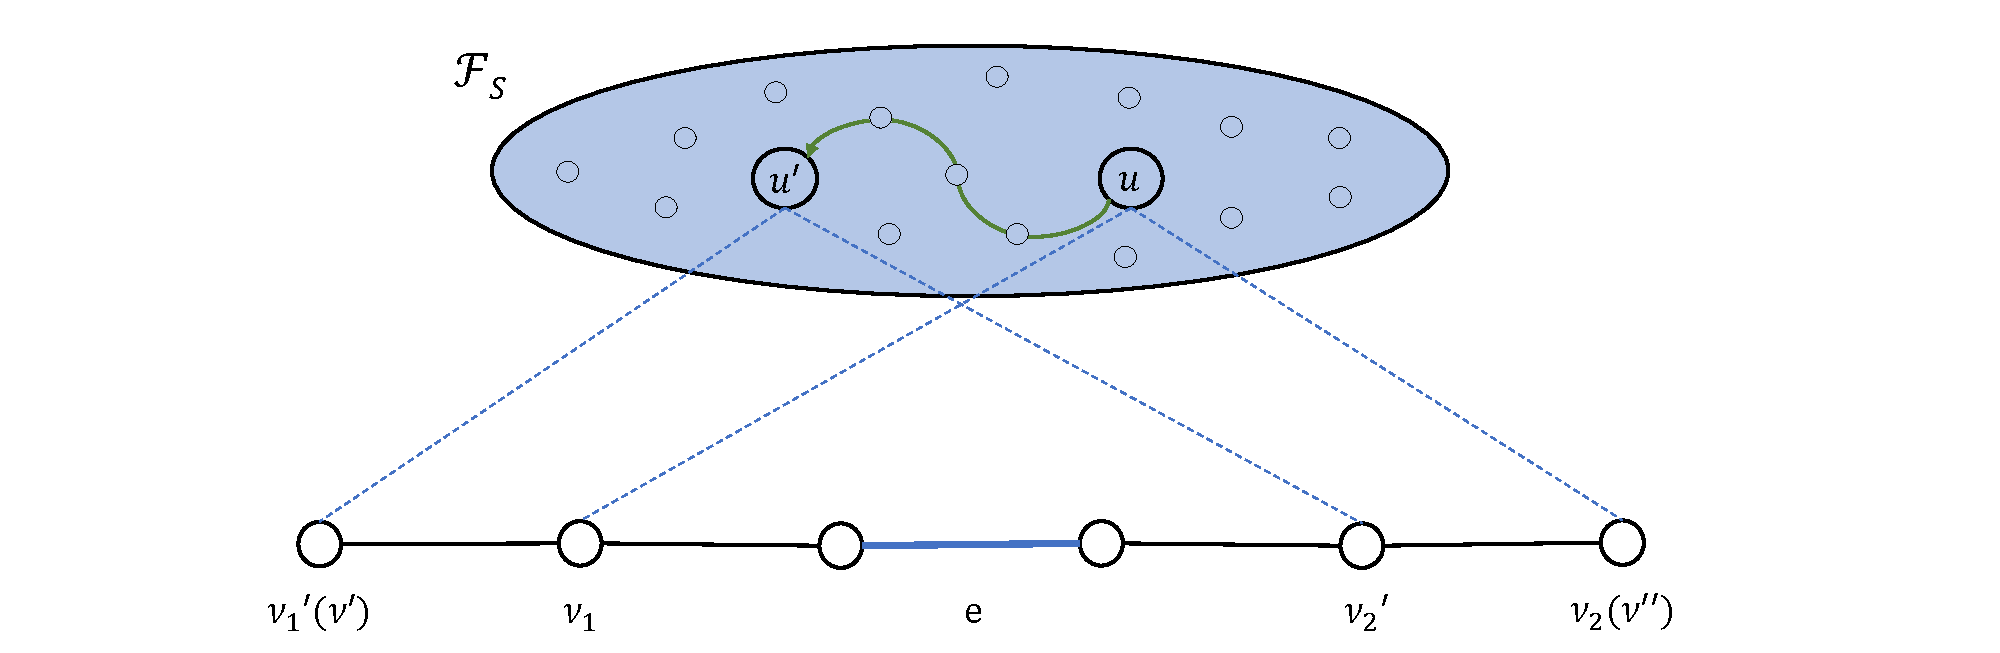
\includegraphics[width=0.95\textwidth]{src/images/proof-reachability-compressed.pdf}
    \caption{The structure of path $P(\nu',\nu'')$.}
\label{fig:structure-of-p(nu',nu'')}
\end{figure}

\end{proof}
% Lemma \ref{lem:contracted-subcactus-mincut} implies that vertex set compressed to each contracted node defines a Steiner mincut. This completes the proof of Lemma \ref{lem:u-u'-in-G-nu}.

Consider the set of non-terminals in the strip ${\cal D}_{s,t}$ that are not compressed to contracted vertex $v_c$. Let this set be $U$. Observe that the set of units $\bigcup_{u\in U} {\cal R}_s(u)$ form a Steiner mincut (using Lemma \ref{lem:reachability-cones}). Moreover, it follows from Lemma \ref{lem:u-u'-in-G-nu} that each non-terminal unit in the set $\bigcup_{u\in U} {\cal R}_s(u)$ is not compressed to contracted vertex $v_c$. Thus, $U = \bigcup_{u\in U} {\cal R}_s(u) \setminus \{\mathbf{s}\}$. All the set of vertices compressed to $v_c$ forms the complement of set $\bigcup_{u\in U} {\cal R}_s(u)$, and thus defines the same Steiner mincut. Therefore, the set of vertices corresponding to each contracted vertex defines a Steiner mincut.

It follows from the construction that $G_{S'}$ is a quotient graph of $G$. Moreover, the number of contracted vertices equals the number of cycles and tree edges incident on node $\nu$ in the skeleton.  We state the following lemma.




% $G_{S'}$ obtained after the $2-$step contraction procedure. 
% that will be required for answering the queries.

\begin{lemma}
Let $S'\subset S$ be a maximal subset of vertices such that $c_{S'}>c_S$ and $\nu$ be the node in ${\cal H}_S$ corresponding to $S'$. Let $G_{S'}$ be the graph obtained after %applying the above procedure.
$2$-step contraction procedure. 
\begin{enumerate}
    \item The set of vertices compressed to a contracted vertex defines a Steiner mincut for set $S$.
    \item The number of contracted vertices equals the number of cycles and tree edges incident on node $\nu$ in ${\cal H}_S$.
\end{enumerate}
\label{lem:contracted-subcactus-mincut}
\end{lemma}


\vspace{-8mm}
\section{Query transformation in \texorpdfstring{$G_{S'}$}{compact graph}}
% {\color{red} Motivation for this subsection is missing in the following start line.}

% The graph $G_{S'}$ does not even contain all edges of graph $G$ because a large portion of vertices is contracted. However, we can use the findings of Section \ref{sec:query-transformation} to effectively handle this problem. 
We begin with a lemma that was used by Gomory and Hu to build a tree storing all-pairs mincuts. 

\begin{lemma}[Gomory and Hu \cite{GH61}]
Let $A$ defines a $(s,t)$-mincut with $s\in A$. Let $r\in A$ be any vertex.
For any $(s,r)$-mincut, say defined by $B$, there exists a $(s,r)$-mincut that keeps $\bar A$ intact and still contains all edges in cut defined by $B$ that don't have both endpoints in $\bar A$.
\label{lem:GH}
\end{lemma}

Consider any two vertices $s,r\in S'$. Recall that $S'$ is mapped to $\nu$ in the skeleton ${\cal H}_S$. 
% Consider any cycle $c$ that passes through $\nu$ in the cactus. 
Let $A$ be the subset of vertices compressed to a contracted vertex in $G_{S'}$. Notice that all those $(s,r)$-mincuts in $G$ that keep $\bar{A}$ intact remain preserved in $G_{S'}$. Moreover, it follows from Lemma \ref{lem:contracted-subcactus-mincut} and Lemma \ref{lem:GH} that there is at least one such $(s,r)$-mincut. So it suffices to work with graph $G_{S'}$ if one wishes to calculate the value of $(s,r)$-mincut in $G$ or simply report a $(s,r)$-mincut in $G$
for any $s,r\in S$. Moreover, we can answer a query \textsc{edge-contained}$(s,r,E_y)$ using $G_{S'}$ if all edges in $E_y$ remain intact in graph $G_{S'}$. 
However, answering a query \textsc{edge-contained}$(s,r,E_{y})$ for any arbitrary $E_y$ using $G_{S'}$ is still challenging. This is because 
% we need to find at least one $(s,r)$-mincut in $G$ that contains all edges in $E_y$ but 
$G_{S'}$ may not even preserve all $(s,r)$-mincuts. In particular, all those $(s,r)$-mincuts that cut the set associated with a contracted vertex in $G_{S'}$ get lost during the transformation from $G$ to $G_{S'}$. We shall now establish a mapping from the set of all such lost $(s,r)$-mincuts to the set of $(s,r)$-mincuts that are present in $G_{S'}$. 

Let $y$ belong to $\bar{A}$. It follows from Lemma \ref{lem:contracted-subcactus-mincut} that the cut $(A,\bar{A})$ is a $(s,t)$-mincut for any $t\in S\cap \bar{A}$. Hence, $A,s,t,r$ satisfy all conditions of Theorem  \ref{thm:query-transform}. Now notice that entire $\bar{A}$
is compressed to a single vertex, say $y'$, in $G_{S'}$. Hence we can state the following Theorem.



\begin{theorem} \label{thm:edge-correspondence}
Given an undirected graph $G=(V,E)$, a subset $S\subseteq V$, let $S'\subset S$ be a maximal subset of vertices such that $c_{S'}>c_S$.
There exists a quotient graph $G_{S'}$ with the following property.~
For any two vertices $r,s \in S'$ and a set of edges $E_y$ incident on vertex $y$ in $G$, there exists a set of edges $E_{y'}$ incident on a vertex $y'$ in $G_{S'}$ such that $E_y$ lies in a $(r,s)$-mincut in $G$ if and only if $E_{y'}$ lies in a $(r,s)$-mincut in $G_{S'}$. 
\end{theorem}

We have already seen the construction of $G_{S'}$. In order to transform  \textsc{edge-contained}$(s,r,E_y)$ to \textsc{edge-contained}$(s,r,E_{y'})$  using Theorem \ref{thm:edge-correspondence}, we give an efficient algorithm for computing $E_{y'}$. Moreover, once we find a $(r,s)$-mincut in $G_{S'}$ that contains $E_{y'}$ we can efficiently compute a $(r,s)$-mincut in $G$ that contains all edges in $E_{y}$. Interestingly, we have algorithms that run in time linear in the size of flesh for both these tasks, stated in the following Lemma. 

\begin{lemma}
\label{lem:linear-time-qt}
Set of edges $E_{y'}$ in Theorem \ref{thm:edge-correspondence} can be obtained from $E_y$ given flesh ${\cal F}_S$ and skeleton $\mathcal H_S$ in time linear in the size of flesh.
\end{lemma}

\begin{lemma}
\label{lem:mincut-qt}
Given a $(r,s)$-mincut in $G_{S'}$ that contains the all edges in set $E_{y'}$, we can construct a $(r,s)$-mincut in $G$ that contains all edges in set $E_y$ in time linear in the size of flesh ${\cal F}_S$.
% (Proof follows from Corollary \ref{cor:query-transformation})
\end{lemma}

\begin{proof}
Consider the case when $y$ does not belong to any contracted vertex. In this case, all edges in $E_y$ remain intact in $G_{S'}$ and thus $E_{y'}=E_{y}$.

Now, suppose $y$ belong to contracted vertex $y'$. Let $\bar A$ be the set of vertices compressed to contracted vertex $y'$. We select a vertex $t\in {\bar A} \cap S$ and construct the ${\cal D}_{A,t}$ strip using the flesh ${\cal F}_S$ and skeleton ${\cal H}_S$ in time linear in the size of flesh (using Lemma \ref{lem:strip-from-carcass}). Using the construction outlined in Lemma \ref{lem:query-transformation} we can obtain the set of edges $E_{A}$ by computing reachability cone(s) in strip ${\cal D}_{A,t}$. This takes time linear in size of ${\cal D}_{A,t}$. All edges in $E_A$ share same endpoint $y'$ in $G_{S'}$. Thus, we get the set of edges $E_{y'}$ which is simply all edges in $G_{S'}$ corresponding to set $E_A$. Clearly, this process can be accomplished in time linear in the size of flesh ${\cal F}_S$.

Suppose we have a $(r,s)$-mincut in $G_{S'}$, say $B$ such that $s,t \not\in B$ that contains all edges in $E_{y'}$. If $y$ does not belong to any contracted vertex, this cut itself can be reported as $E_y=E_{y'}$. Suppose $y$ belong to contracted vertex $y'$. We can construct another $(r,s)$-mincut $B\cup R$ (recall the definition of $R$ in Proof of Lemma \ref{lem:query-transformation}). This procedure also involves construction of ${\cal D}_{A,t}$ strip and computation of reachability cone(s) in this strip. This process can also be accomplished in time linear in the size of flesh ${\cal F}_S$.
\end{proof}